\documentclass{article}
\usepackage{graphicx}
\usepackage[margin=1.5cm]{geometry}
\usepackage{amsmath}

\begin{document}

\title{Warm Up: Kinematics in 2D and 3D}
\author{Prof. Jordan C. Hanson}

\maketitle

\section{Memory}

\begin{enumerate}
\item $\vec{v} = \Delta \vec{x}/\Delta t$ ... Average velocity.
\item $\Delta \vec{x} = \vec{v} \Delta t$ ... Rearranged, solved for displacement.
\item $y(t) = -\frac{1}{2}g t^2 + v_{i,y}t + y_i$ ... Displacement if constantly accelerating with $-g$.
\item $v(t) = -g t + v_{i}$ ... Velocity equation if there is constant acceleration.
\end{enumerate}

\section{Kinematics in 2D and 3D}

\begin{enumerate}
\item Imagine a system propagating through 3D space with a position vector $\vec{x} = (2t^2-t)\hat{i} + 2t\hat{j}$.  (a) What is the average velocity between $t = 0$ and $t = 2$ seconds? (b) If the object starts at the origin at $t = 0$, what is the displacement at $t = 2$?  (c) What angle does the displacement make with the x-axis? \\ \vspace{1cm}
\item Suppose a system is thrown straight up into the air.  The initial vertical velocity is $v_{i,y} = 10$ m/s.
\begin{itemize}
\item What is the speed at the apex of the trajectory? \\ \vspace{1cm}
\item How long does the system spend in the air? \\ \vspace{1cm}
\item Consider the same system, but now the initial velocity is at a 45 degree angle with respect to the horizontal.  If $v_i = 10$ m/s, this means that $v_{i,y}$, the vertical component of the initial velocity, is not 10 m/s (see Fig. \ref{fig:1}).
\item How long does the system spend in the air?
\end{itemize}
\end{enumerate}

\begin{figure}[hb]
\centering
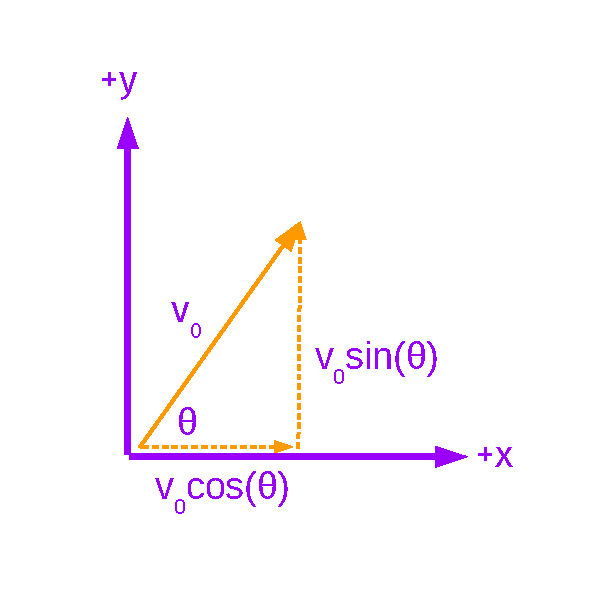
\includegraphics[width=0.3\textwidth,trim=0cm 1cm 0cm 1cm,clip=true]{figures/Vectors1.pdf}
\caption{\label{fig:1} The initial velocity, if tilted at an angle, broken into components.}
\end{figure}

\end{document}
